\section{Accessibilità}
\subsection{Colori}


\subsection{Navigazione nel sito}
Una semplice navigazione nel sito è garantita, in primo luogo, da una semplice \textit{navbar} che non include sottomenù. Sono direttamente visibili e accessibili tutte le pagine del sito web:
\begin{figure}[h]
		\begin{center}
		
\includegraphics[scale=0.3]{Images/headerSito.png}
		\caption{Header del sito, in particolare visto dalla home page.}
	\end{center}
\end{figure}\\
Inoltre, il posizionamento corrente all'interno del sito web è chiarito grazie all'evidenziazione della pagina corrente all'interno della navbar:
\begin{figure}[h]
	\begin{center}
		
\includegraphics[scale=0.2]{Images/selezionePaginaCorrente.png}
		\caption{Dettaglio: la pagina corrente è evidenziata rispetto alle altre.}
	\end{center}
\end{figure}\\
Oltre a ciò, sotto l'intestazione del sito è presente l'indicazione testuale sulla corrente posizione all'interno del sito ("\textit{breadcrumbs}"):
\begin{figure}[h]
	\begin{center}
		
\includegraphics[scale=0.6]{Images/breadcrumbs.png}
		\caption{Dettaglio: \textit{breadcrumbs}.}
	\end{center}
\end{figure}\\
Per quanto concerne i link presenti nel sito, è stato fatto in modo che link "\textit{visitati}" e "ancora da visitare" siano facilmente distinguibili. Un esempio è visibile nella figura \ref{fig:linkVisitatiDaVisitare}.
\begin{figure}[h]
	\begin{center}
		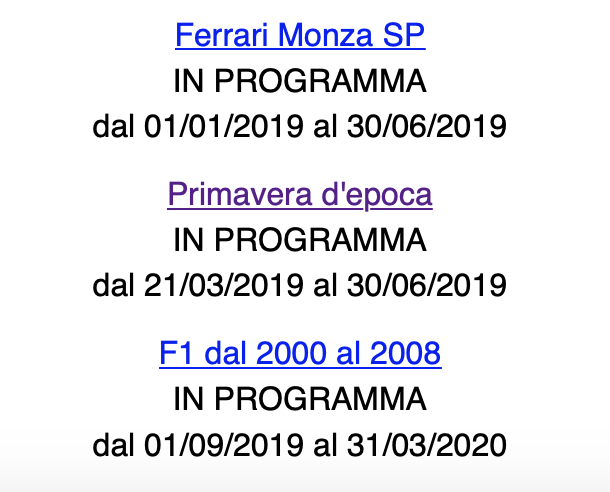
\includegraphics[scale=0.3]{Images/linkVisitatiDaVisitare.png}
		\caption{Dettaglio: link da visitare e visitati. Il link centrale è stato già visitato mentre il primo e l'ultimo risultano ancora da esplorare.}
		\label{fig:linkVisitatiDaVisitare}
	\end{center}
\end{figure}\\
Per rendere efficiente la navigazione all'interno del sito anche ad utenti con difficoltà visive, è stato fatto uso di \textit{tabindex} per consentire un'agile navigazione all'interno del sito. Ogni immagine è inoltre accompagnata da un \textit{alt} che descriva in modo soddisfacente l'immagine in oggetto.\\
È stato inoltre inserito un bottone che consente di tornare facilmente in testa alla pagina.

\subsection{Mobile}